\documentclass{article}
\usepackage{../../Self_Style}

\title{Hatcher Chapter 0 Notes}
\author{Zih-Yu Hsieh}
\date{\today}

\begin{document}
\maketitle

\tableofcontents

\section{Retraction, Homotopy, and Deformation Retraction}

This part is mainly a review of the definitions I know:

This part is mainly ways of classifying the spaces with similar shapes, with the definition much broader than homeomorphis (which is too strict).

\begin{defn}[Retraction]
    Given a subspace $A \subset.eq X$, a \textbf{Retraction} of $X$ onto $A$, is a continuous map $r:X \rightarrow X$, such that $r(X)=A$, and the restriction $r\big|_{A} = \id_{A}$.

    \hfil

    A more formal definition can be viewed as a continuous idempotent map, or  $r:X\rightarrow X$ satisfies $r^2=r$.
\end{defn}

Here are some examples:
\begin{exm}
    Every constant map is a trivial example of retraction, since $r:X\rightarrow X$ by $r(x)=x_0$ for all $x\in X$ (given some $x_0\in X$) is continuous, $r^2=r$, and is an identity on $x_0$ itself.
\end{exm}

\begin{exm}
    $\RR^2\setminus\{0\}$ has a retraction onto $S^1$, by the map $r:\RR^2\setminus\{0\}\rightarrow\RR^2\setminus\{0\}$, $r(\bar{x}) = \frac{\bar{x}}{\|\bar{x}\|}$. (In fact, this is coming from a deformation retraction).
\end{exm}

However, \textbf{Example 1} is an example that retraction is too broad as a definition, since every nonempty space has a retraction to a singleton. So, the classification of ``space with similar shape'' needs to be broaden.

For this, it requires a notion of ``deformation'' on continuous maps:
\begin{defn}[Homotopy]
    A \textbf{Homotopy} between two continuous maps $f_0,f_1:X\rightarrow Y$, is a continuous map $F:X \times I\rightarrow Y$, such that every $x\in X$, one has $f(x,0) = f_0(x)$, and $f(x,1) = f_1(x)$.

    Which, for all $t\in[0,1]$, the map $f_t:X\rightarrow Y$ is defined as $f_t(x):= f(x,t)$.

    Which, we say $f,g$ are \textbf{Homotopic}, denotes as $f\simeq g$.
\end{defn}

Which, it's known that homotopy is an equivalence relation on the set of continuous maps.

\hfil

Now, sometimes homotopy needs extra requirements: For instance, having the homotopy be independent on some subspace. Which leads to the following definition:
\begin{defn}[]
    Given a subset $A\subseteq X$, $F:X\times I\rightarrow Y$ a homotopy. $F$ is called a \textbf{Homotopy Relative to } $A$, if for any $t\in[0,1]$, $f_t\big|_A = f_0\big|_A$.  In other words, the homotopy remains fixed on $A$.
\end{defn}

As an example, one can see the following:

\begin{exm}
    The map $r:\RR^2\setminus\{0\}\rightarrow\RR^2\setminus\{0\}$ by $r(\bar{x}) = \frac{\bar{x}}{\|\bar{x}\|}$ is in fact homotopic to the identity map; moreover, it's homotopic relative to $S^1$. Which, can be constructed as follow:

    Let $X:= \RR^2\setminus\{0\}$, define $F:X\times I\rightarrow X$ by $F(\bar{x}, t):= \frac{t\bar{x}}{\|\bar{x}\|} + (1-t)\bar{x}$. Which, it's clearly continuous. Also, one has $f_0(\bar{x}) = \bar{x}$ (identity), and $f_1(\bar{x}) = \frac{\bar{x}}{\|\bar{x}\|}$ ($r$). 
    
    Finally, for all $\bar{x}\in S^1$, since $\|\bar{x}\|=1$, then one has $f_t(\bar{x}) = t\bar{x} + (1-t)\bar{x} = \bar{x}$, it's identity on $S^1$.
\end{exm}

\hfil

Now, in case to deal with deformation within the space itself, one combines the two definition above:
\begin{defn}[Deformation Retraction]
    Given $A\subseteq X$, a \textbf{Deformation Retraction} of a space $X$ onto a subspace $A$, is a homotopy $F:X\times I\rightarrow X$, such that $f_0 = \id_X$, while $f_1:X\rightarrow X$ is a retraction onto $A$. Also, it's required that $f_t\big|_A = \id_A$ for all $t\in[0,1]$.
\end{defn}

The above \textbf{Example 3} shows that $r$ is a deformation retraction, instead of just a retraction.

Finally, this gives rise to a new definition:
\begin{defn}[Mapping Cylinder]
    Given a map $f:X \rightarrow Y$, the \textbf{Mapping Cylinder} $M_f$ is the quotient space of the disjoint union $(X\times I)\sqcup Y$, obtained by $(x,1) \sim f(x)$ for all $x\in X$.
\end{defn}

Here is an illustration about Mapping Cylinder:
\begin{figure}[h!]
    \centering
    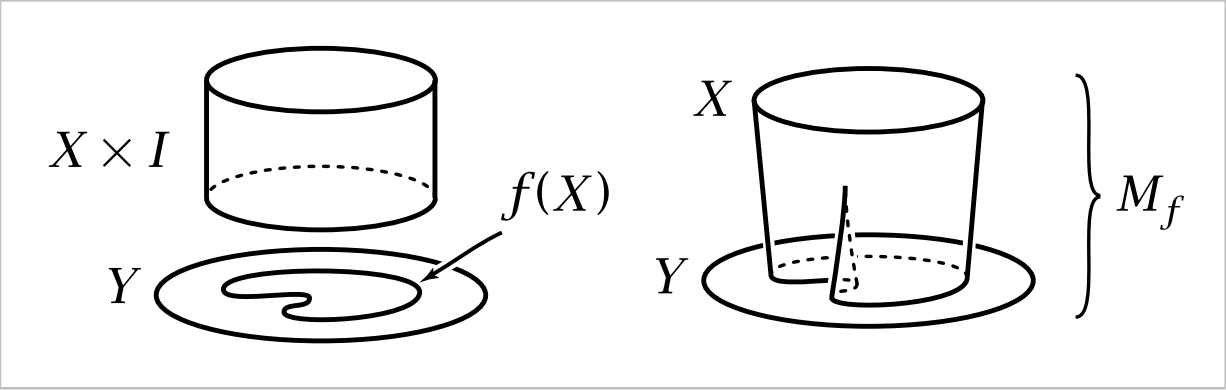
\includegraphics[width=100mm]{Mapping Cylinder.png}
\end{figure}
Which, the mapping cylinder satisfies some properties:
\begin{prop}
    The Mapping Cylinder $M_f$ deformation retracts onto the subspace $Y$.
\end{prop}
\begin{proof}
    Define a continuous map $F:M_f\times I\rightarrow M_f$ as follow:
    \begin{itemize}
        \item For $y \in Y$, define $F(y,s) = y$ for all $s\in[0,1]$ (which, for all $x\in X$, one has $f(x)\sim (x,1)$ in $M_f$).
        \item For $t\in [0,1)$ and $s\in [0,1]$, define $F((x,t), s) = (x,s + (1-s)t)$.
    \end{itemize}
    Which, the map is continuous (check Hatcher Appendix A.17, which claims that if $f:X\rightarrow Y$ is a quotient map, with $Z$ being locally compact, then $f \times \id_Z:X \times Z\rightarrow Y\times Z$ is a quotient map). When $s=0$, one has $F(y,0) = y$ and $F((x,t),0) = (x,t)$ for $t<1$; also for $s=1$, one has $F(y,1)=y$ and $F((x,t),1) = (x,t) = f(x)$. Finally, it's stationary on $Y$ by the definition, hence it deformation retracts onto $Y$.
\end{proof}

Finally, a relation on the spaces can be given using homotopy:
\begin{defn}{Homotopy Equivalence}
    A continuous map $f:X\rightarrow Y$ is a \textbf{Homotopy Equivalence}, if there exists continuous map $g:Y\rightarrow X$, such that $g \circ f\simeq \id_X$, and $f\circ g\simeq \id_Y$.

    Which, in this case it's said that $X$ and $Y$ are \textbf{Homotopy Equivalent}, or having the same \textbf{Homotopy Type}, which is denoted as $X\simeq Y$.
\end{defn}

Which, here it can give a specific definition of space with stronger connectedness:
\begin{defn}[Contractable Space]
    A space is called \textbf{Contractable}, if it is homotopy equivalent to a singleton. 

    Which, having the identity map being homotopic to a constant map is sufficient.
\end{defn}

\textbf{Question:} Is the above definition an equivalence relation?

As a side note,  being contractable may be a bit different from simply-connected space, since there are spaces where it's contractable, but maybe not path-connected.

\newpage

\section{Cell Complexes}

\end{document}